\documentclass[tikz,border=6pt]{standalone}
\usepackage{amsmath,amssymb}
\usepackage{xcolor}
\definecolor{accent}{HTML}{A13D2C}
\definecolor{accent2}{HTML}{2B5F6B}
\definecolor{muted}{HTML}{5A564F}
\definecolor{linecol}{HTML}{D8D2C4}
\definecolor{astroblue}{HTML}{1B4F72}
\usetikzlibrary{arrows.meta}
\usepackage[T1]{fontenc}\usepackage{newpxtext,newpxmath}  % same fonts as the notes
\begin{document}
% A ring of free particles under a wave travelling along z (out of the page).
% Each displaced position is (Id + 1/2 [[h+, hx],[hx, -h+]]) (cos phi, sin phi), with h0 = 0.4 (exaggerated).
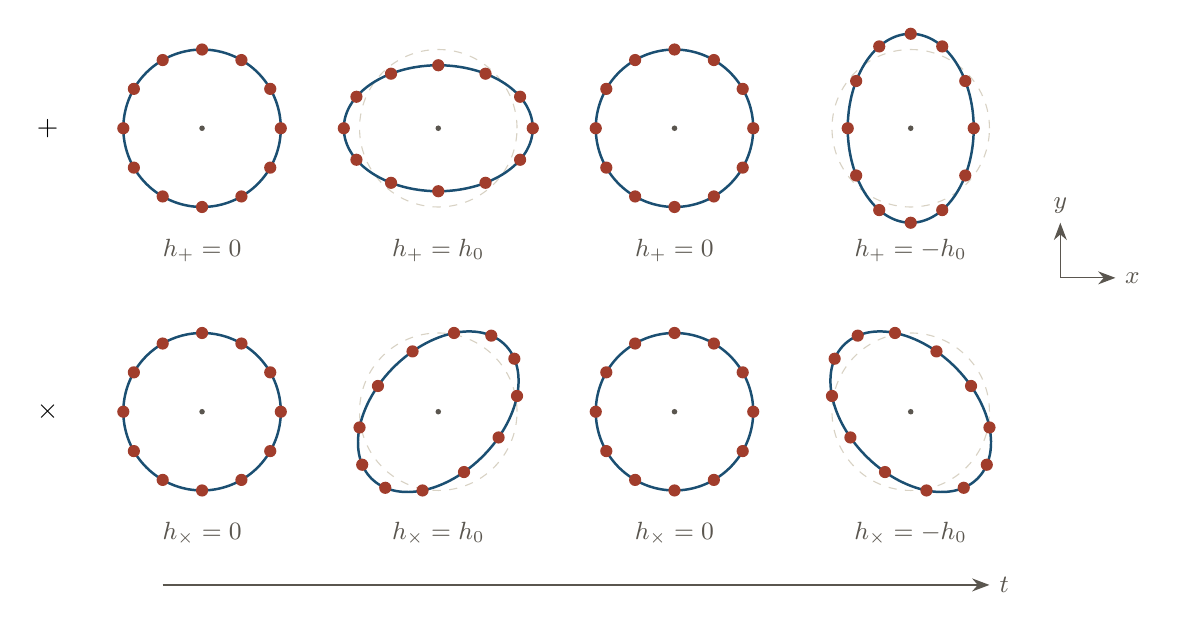
\begin{tikzpicture}[x=1cm,y=1cm, >={Stealth[length=2.2mm]}]
  \def\hO{0.4}
  % #1 column x, #2 row y, #3 h+, #4 hx, #5 label
  \newcommand{\ring}[5]{%
    \begin{scope}[shift={(#1,#2)}]
      \draw[linecol, dashed] (0,0) circle[radius=1];
      \draw[astroblue, line width=0.9pt] plot[domain=0:360, samples=73, smooth]
        ({(1+#3/2)*cos(\x)+(#4/2)*sin(\x)}, {(#4/2)*cos(\x)+(1-#3/2)*sin(\x)});
      \foreach \p in {0,30,...,330}
        \fill[accent] ({(1+#3/2)*cos(\p)+(#4/2)*sin(\p)}, {(#4/2)*cos(\p)+(1-#3/2)*sin(\p)}) circle[radius=2.2pt];
      \fill[muted] (0,0) circle[radius=1pt];
      \node[muted] at (0,-1.55) {\small #5};
    \end{scope}}
  % top row: plus polarisation
  \ring{0}{0}{0}{0}{$h_+=0$}
  \ring{3}{0}{\hO}{0}{$h_+=h_0$}
  \ring{6}{0}{0}{0}{$h_+=0$}
  \ring{9}{0}{-\hO}{0}{$h_+=-h_0$}
  % bottom row: cross polarisation
  \ring{0}{-3.6}{0}{0}{$h_\times=0$}
  \ring{3}{-3.6}{0}{\hO}{$h_\times=h_0$}
  \ring{6}{-3.6}{0}{0}{$h_\times=0$}
  \ring{9}{-3.6}{0}{-\hO}{$h_\times=-h_0$}
  % row titles and axes
  \node[anchor=east] at (-1.7,0) {$+$};
  \node[anchor=east] at (-1.7,-3.6) {$\times$};
  \draw[->, muted] (10.9,-1.9) -- (11.6,-1.9) node[right] {\small $x$};
  \draw[->, muted] (10.9,-1.9) -- (10.9,-1.2) node[above] {\small $y$};
  \draw[->, muted, line width=0.6pt] (-0.5,-5.8) -- (10,-5.8) node[right] {\small $t$};
\end{tikzpicture}
\end{document}
